\documentclass{standalone}
\usepackage{tikz}
\usetikzlibrary{patterns, positioning}

\begin{document}
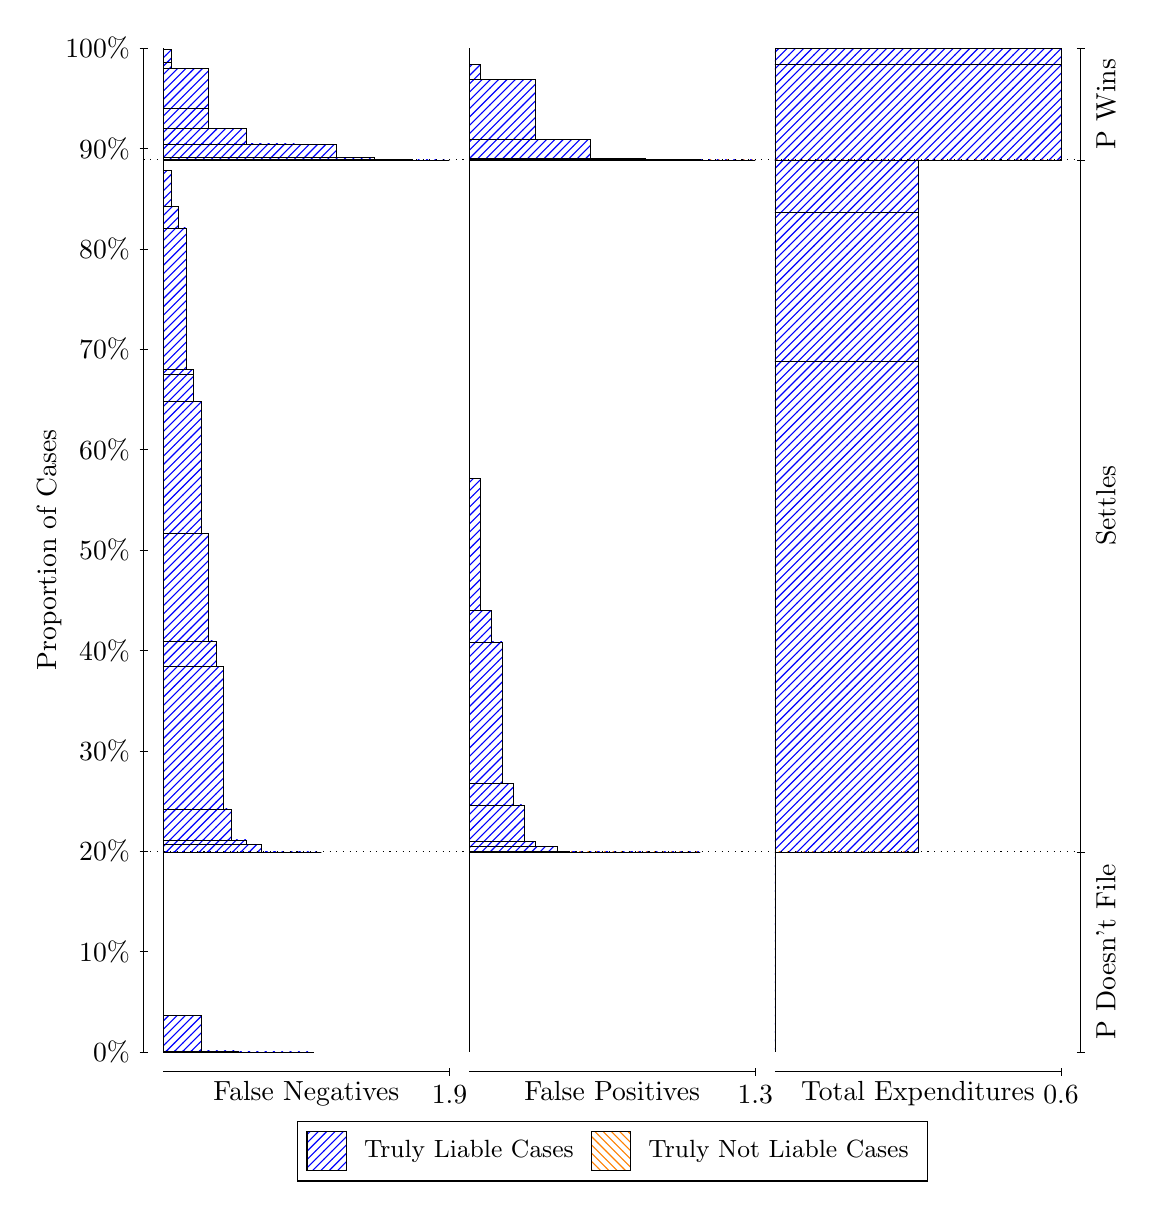
\begin{tikzpicture}
\draw[black, very thin] (1.5,1.75) -- (1.5,14.5);
\node[rotate=90, anchor=center] at (0.3, 8.125) {Proportion of Cases};
\draw[black, very thin] (1.45,1.75) -- (1.55,1.75);
\node[anchor=east] at (1.45, 1.75) {0\%};
\draw[black, very thin] (1.45,3.025) -- (1.55,3.025);
\node[anchor=east] at (1.45, 3.025) {10\%};
\draw[black, very thin] (1.45,4.3) -- (1.55,4.3);
\node[anchor=east] at (1.45, 4.3) {20\%};
\draw[black, very thin] (1.45,5.575) -- (1.55,5.575);
\node[anchor=east] at (1.45, 5.575) {30\%};
\draw[black, very thin] (1.45,6.85) -- (1.55,6.85);
\node[anchor=east] at (1.45, 6.85) {40\%};
\draw[black, very thin] (1.45,8.125) -- (1.55,8.125);
\node[anchor=east] at (1.45, 8.125) {50\%};
\draw[black, very thin] (1.45,9.4) -- (1.55,9.4);
\node[anchor=east] at (1.45, 9.4) {60\%};
\draw[black, very thin] (1.45,10.675) -- (1.55,10.675);
\node[anchor=east] at (1.45, 10.675) {70\%};
\draw[black, very thin] (1.45,11.95) -- (1.55,11.95);
\node[anchor=east] at (1.45, 11.95) {80\%};
\draw[black, very thin] (1.45,13.225) -- (1.55,13.225);
\node[anchor=east] at (1.45, 13.225) {90\%};
\draw[black, very thin] (1.45,14.5) -- (1.55,14.5);
\node[anchor=east] at (1.45, 14.5) {100\%};

\draw[black, very thin] (13.4,1.75) -- (13.4,14.5);
\draw[black, very thin] (13.35,1.75) -- (13.45,1.75);
\node[anchor=west] at (13.35, 1.75) {};
\draw[black, very thin] (13.35,4.2923) -- (13.45,4.2923);
\node[anchor=west] at (13.35, 4.2923) {};
\draw[black, very thin] (13.35,13.08) -- (13.45,13.08);
\node[anchor=west] at (13.35, 13.08) {};
\draw[black, very thin] (13.35,14.5) -- (13.45,14.5);
\node[anchor=west] at (13.35, 14.5) {};

\draw[black, very thin, pattern color=blue, pattern=north east lines] (1.75,1.75) rectangle (3.6623,1.75);
\draw[black, very thin, pattern color=blue, pattern=north east lines] (1.75,1.75) rectangle (3.1842,1.7501);
\draw[black, very thin, pattern color=blue, pattern=north east lines] (1.75,1.7501) rectangle (2.7061,1.764);
\draw[black, very thin, pattern color=blue, pattern=north east lines] (1.75,1.764) rectangle (2.2281,2.2108);
\draw[black, very thin, pattern color=orange, pattern=north west lines] (1.75,2.2108) rectangle (1.75,2.2108);
\draw[black, very thin, pattern color=blue, pattern=north east lines] (1.75,2.2108) rectangle (1.75,4.2923);
\draw[black, very thin, pattern color=blue, pattern=north east lines] (1.75,4.2923) rectangle (3.7579,4.2923);
\draw[black, very thin, pattern color=blue, pattern=north east lines] (1.75,4.2923) rectangle (3.5667,4.2923);
\draw[black, very thin, pattern color=blue, pattern=north east lines] (1.75,4.2923) rectangle (3.3754,4.2923);
\draw[black, very thin, pattern color=blue, pattern=north east lines] (1.75,4.2923) rectangle (3.2798,4.2923);
\draw[black, very thin, pattern color=blue, pattern=north east lines] (1.75,4.2923) rectangle (3.0886,4.2923);
\draw[black, very thin, pattern color=blue, pattern=north east lines] (1.75,4.2923) rectangle (2.993,4.383);
\draw[black, very thin, pattern color=blue, pattern=north east lines] (1.75,4.383) rectangle (2.8974,4.3858);
\draw[black, very thin, pattern color=blue, pattern=north east lines] (1.75,4.3858) rectangle (2.8018,4.4445);
\draw[black, very thin, pattern color=blue, pattern=north east lines] (1.75,4.4445) rectangle (2.6105,4.8347);
\draw[black, very thin, pattern color=blue, pattern=north east lines] (1.75,4.8347) rectangle (2.6105,4.838);
\draw[black, very thin, pattern color=blue, pattern=north east lines] (1.75,4.838) rectangle (2.5149,6.6427);
\draw[black, very thin, pattern color=blue, pattern=north east lines] (1.75,6.6427) rectangle (2.4193,6.9709);
\draw[black, very thin, pattern color=blue, pattern=north east lines] (1.75,6.9709) rectangle (2.3237,8.3362);
\draw[black, very thin, pattern color=blue, pattern=north east lines] (1.75,8.3362) rectangle (2.2281,10.015);
\draw[black, very thin, pattern color=blue, pattern=north east lines] (1.75,10.015) rectangle (2.1325,10.353);
\draw[black, very thin, pattern color=blue, pattern=north east lines] (1.75,10.353) rectangle (2.1325,10.416);
\draw[black, very thin, pattern color=blue, pattern=north east lines] (1.75,10.416) rectangle (2.0368,12.216);
\draw[black, very thin, pattern color=blue, pattern=north east lines] (1.75,12.216) rectangle (1.9412,12.486);
\draw[black, very thin, pattern color=blue, pattern=north east lines] (1.75,12.486) rectangle (1.8456,12.944);
\draw[black, very thin, pattern color=orange, pattern=north west lines] (1.75,12.944) rectangle (1.75,12.944);
\draw[black, very thin, pattern color=blue, pattern=north east lines] (1.75,12.944) rectangle (1.75,13.08);
\draw[black, very thin, pattern color=blue, pattern=north east lines] (1.75,13.08) rectangle (5.3833,13.08);
\draw[black, very thin, pattern color=blue, pattern=north east lines] (1.75,13.08) rectangle (4.9053,13.081);
\draw[black, very thin, pattern color=blue, pattern=north east lines] (1.75,13.081) rectangle (4.4272,13.108);
\draw[black, very thin, pattern color=blue, pattern=north east lines] (1.75,13.108) rectangle (3.9491,13.272);
\draw[black, very thin, pattern color=blue, pattern=north east lines] (1.75,13.272) rectangle (3.7579,13.272);
\draw[black, very thin, pattern color=blue, pattern=north east lines] (1.75,13.272) rectangle (3.4711,13.284);
\draw[black, very thin, pattern color=blue, pattern=north east lines] (1.75,13.284) rectangle (3.2798,13.284);
\draw[black, very thin, pattern color=blue, pattern=north east lines] (1.75,13.284) rectangle (2.993,13.284);
\draw[black, very thin, pattern color=blue, pattern=north east lines] (1.75,13.284) rectangle (2.8018,13.479);
\draw[black, very thin, pattern color=blue, pattern=north east lines] (1.75,13.479) rectangle (2.5149,13.479);
\draw[black, very thin, pattern color=blue, pattern=north east lines] (1.75,13.479) rectangle (2.3237,13.737);
\draw[black, very thin, pattern color=blue, pattern=north east lines] (1.75,13.737) rectangle (2.3237,14.244);
\draw[black, very thin, pattern color=blue, pattern=north east lines] (1.75,14.244) rectangle (1.8456,14.324);
\draw[black, very thin, pattern color=blue, pattern=north east lines] (1.75,14.324) rectangle (1.8456,14.484);
\draw[black, very thin, pattern color=orange, pattern=north west lines] (1.75,14.484) rectangle (1.75,14.484);
\draw[black, very thin, pattern color=blue, pattern=north east lines] (1.75,14.484) rectangle (1.75,14.5);
\draw[black, very thin, pattern color=orange, pattern=north west lines] (5.6333,1.75) rectangle (5.6333,1.75);
\draw[black, very thin, pattern color=blue, pattern=north east lines] (5.6333,1.75) rectangle (5.6333,4.2923);
\draw[black, very thin, pattern color=orange, pattern=north west lines] (5.6333,4.2923) rectangle (8.5679,4.2923);
\draw[black, very thin, pattern color=blue, pattern=north east lines] (5.6333,4.2923) rectangle (8.5679,4.2923);
\draw[black, very thin, pattern color=orange, pattern=north west lines] (5.6333,4.2923) rectangle (8.009,4.2923);
\draw[black, very thin, pattern color=blue, pattern=north east lines] (5.6333,4.2923) rectangle (8.009,4.2923);
\draw[black, very thin, pattern color=blue, pattern=north east lines] (5.6333,4.2923) rectangle (7.8692,4.2923);
\draw[black, very thin, pattern color=orange, pattern=north west lines] (5.6333,4.2923) rectangle (7.45,4.2923);
\draw[black, very thin, pattern color=blue, pattern=north east lines] (5.6333,4.2923) rectangle (7.45,4.2923);
\draw[black, very thin, pattern color=blue, pattern=north east lines] (5.6333,4.2923) rectangle (7.3103,4.2923);
\draw[black, very thin, pattern color=blue, pattern=north east lines] (5.6333,4.2923) rectangle (7.1705,4.2923);
\draw[black, very thin, pattern color=orange, pattern=north west lines] (5.6333,4.2923) rectangle (6.891,4.2923);
\draw[black, very thin, pattern color=blue, pattern=north east lines] (5.6333,4.2923) rectangle (6.891,4.2931);
\draw[black, very thin, pattern color=blue, pattern=north east lines] (5.6333,4.2931) rectangle (6.7513,4.3575);
\draw[black, very thin, pattern color=orange, pattern=north west lines] (5.6333,4.3575) rectangle (6.6115,4.3575);
\draw[black, very thin, pattern color=blue, pattern=north east lines] (5.6333,4.3575) rectangle (6.6115,4.3651);
\draw[black, very thin, pattern color=blue, pattern=north east lines] (5.6333,4.3651) rectangle (6.4718,4.4283);
\draw[black, very thin, pattern color=orange, pattern=north west lines] (5.6333,4.4283) rectangle (6.3321,4.4283);
\draw[black, very thin, pattern color=blue, pattern=north east lines] (5.6333,4.4283) rectangle (6.3321,4.8873);
\draw[black, very thin, pattern color=blue, pattern=north east lines] (5.6333,4.8873) rectangle (6.1923,5.157);
\draw[black, very thin, pattern color=blue, pattern=north east lines] (5.6333,5.157) rectangle (6.0526,6.9568);
\draw[black, very thin, pattern color=blue, pattern=north east lines] (5.6333,6.9568) rectangle (5.9128,7.3577);
\draw[black, very thin, pattern color=blue, pattern=north east lines] (5.6333,7.3577) rectangle (5.7731,9.0366);
\draw[black, very thin, pattern color=blue, pattern=north east lines] (5.6333,9.0366) rectangle (5.6333,13.08);
\draw[black, very thin, pattern color=orange, pattern=north west lines] (5.6333,13.08) rectangle (9.2667,13.08);
\draw[black, very thin, pattern color=blue, pattern=north east lines] (5.6333,13.08) rectangle (9.2667,13.08);
\draw[black, very thin, pattern color=orange, pattern=north west lines] (5.6333,13.08) rectangle (8.5679,13.08);
\draw[black, very thin, pattern color=blue, pattern=north east lines] (5.6333,13.08) rectangle (8.5679,13.081);
\draw[black, very thin, pattern color=orange, pattern=north west lines] (5.6333,13.081) rectangle (7.8692,13.081);
\draw[black, very thin, pattern color=blue, pattern=north east lines] (5.6333,13.081) rectangle (7.8692,13.096);
\draw[black, very thin, pattern color=orange, pattern=north west lines] (5.6333,13.096) rectangle (7.1705,13.096);
\draw[black, very thin, pattern color=blue, pattern=north east lines] (5.6333,13.096) rectangle (7.1705,13.337);
\draw[black, very thin, pattern color=blue, pattern=north east lines] (5.6333,13.337) rectangle (6.4718,14.102);
\draw[black, very thin, pattern color=orange, pattern=north west lines] (5.6333,14.102) rectangle (6.1923,14.102);
\draw[black, very thin, pattern color=blue, pattern=north east lines] (5.6333,14.102) rectangle (6.1923,14.102);
\draw[black, very thin, pattern color=blue, pattern=north east lines] (5.6333,14.102) rectangle (5.7731,14.296);
\draw[black, very thin, pattern color=orange, pattern=north west lines] (5.6333,14.296) rectangle (5.6333,14.296);
\draw[black, very thin, pattern color=blue, pattern=north east lines] (5.6333,14.296) rectangle (5.6333,14.5);
\draw[black, very thin, pattern color=orange, pattern=north west lines] (9.5167,1.75) rectangle (9.5167,1.75);
\draw[black, very thin, pattern color=blue, pattern=north east lines] (9.5167,1.75) rectangle (9.5167,4.2923);
\draw[black, very thin, pattern color=orange, pattern=north west lines] (9.5167,4.2923) rectangle (11.333,4.2923);
\draw[black, very thin, pattern color=blue, pattern=north east lines] (9.5167,4.2923) rectangle (11.333,10.525);
\draw[black, very thin, pattern color=orange, pattern=north west lines] (9.5167,10.525) rectangle (11.333,10.525);
\draw[black, very thin, pattern color=blue, pattern=north east lines] (9.5167,10.525) rectangle (11.333,12.408);
\draw[black, very thin, pattern color=orange, pattern=north west lines] (9.5167,12.408) rectangle (11.333,12.408);
\draw[black, very thin, pattern color=blue, pattern=north east lines] (9.5167,12.408) rectangle (11.333,13.08);
\draw[black, very thin, pattern color=orange, pattern=north west lines] (9.5167,13.08) rectangle (13.15,13.08);
\draw[black, very thin, pattern color=blue, pattern=north east lines] (9.5167,13.08) rectangle (13.15,14.296);
\draw[black, very thin, pattern color=orange, pattern=north west lines] (9.5167,14.296) rectangle (13.15,14.296);
\draw[black, very thin, pattern color=blue, pattern=north east lines] (9.5167,14.296) rectangle (13.15,14.5);
\draw[black, dotted] (1.5,4.2923) -- (13.4,4.2923);
\draw[black, dotted] (1.5,13.08) -- (13.4,13.08);
\draw[black, very thin] (1.75,1.5) -- (5.3833,1.5);
\node[anchor=north] at (3.5667, 1.5) {False Negatives};
\draw[black, very thin] (5.3833,1.45) -- (5.3833,1.55);
\node[anchor=north] at (5.3833, 1.45) {1.9};

\draw[black, very thin] (5.6333,1.5) -- (9.2667,1.5);
\node[anchor=north] at (7.45, 1.5) {False Positives};
\draw[black, very thin] (9.2667,1.45) -- (9.2667,1.55);
\node[anchor=north] at (9.2667, 1.45) {1.3};

\draw[black, very thin] (9.5167,1.5) -- (13.15,1.5);
\node[anchor=north] at (11.333, 1.5) {Total Expenditures};
\draw[black, very thin] (13.15,1.45) -- (13.15,1.55);
\node[anchor=north] at (13.15, 1.45) {0.6};

\node[black, centered, rotate=90] at (13.72, 3.0212) {P Doesn't File};
\node[black, centered, rotate=90] at (13.72, 8.6864) {Settles};
\node[black, centered, rotate=90] at (13.72, 13.79) {P Wins};

\draw (7.449999999999999,1.5) node[draw=none] (baseCoordinate) {};
\begin{scope}[align=center]
        \matrix[scale=0.5, draw=black, below=0.5cm of baseCoordinate, nodes={draw}, column sep=0.1cm]{
            \node[rectangle, draw, minimum width=0.5cm, minimum height=0.5cm, pattern=north east lines, pattern color=blue] {}; &
            \node[draw=none, font=\small] (B) {Truly Liable Cases}; &
            \node[rectangle, draw, minimum width=0.5cm, minimum height=0.5cm, pattern=north west lines, pattern color=orange] {}; &
            \node[draw=none, font=\small] (B) {Truly Not Liable Cases}; \\
            };
\end{scope}

\end{tikzpicture}
\end{document}